\icode{E-MI-SI-L3-261104-002}
如图所示，固定的倾斜光滑杆上套有一个重环，绕过光滑的定滑轮的轻绳一端与重环相连，另一端施加拉力\(F\)使重环从\(A\)点缓慢上升到\(B\)点。设杆对重环的弹力大小为\(F_N\)，整个装置处于同一竖直平面内，在此过程中\paren[]

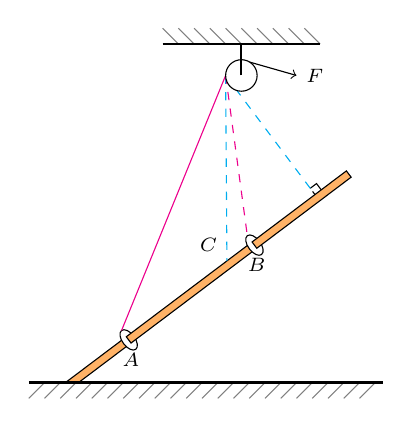
\begin{tikzpicture}[font=\scriptsize]
	\begin{scope}[rotate=37]
		\coordinate (A) at(1,.2);
		\coordinate (B) at(3,.2);
		\coordinate (C) at(4,.1);
		\coordinate (D) at(2.6,.1);
		\draw[fill=orange!60] (0,0) rectangle(1,.1);
		\draw[fill=white] (1,.05) ellipse(.08 and .15);
		\draw[fill=orange!60] (1,0) rectangle (3,0.1);
		\draw[fill=white] (3,.05) ellipse(.08 and .15);
		\draw[fill=orange!60] (3,0) rectangle(4.5,.1);
		\draw (4.1,.1)--(4.1,.2)--(4,.2) (4,.1)--(4,.15);
		\node at(1,0)[below]{\(A\)};
		\node at(3,0)[below]{\(B\)};
	\end{scope}
	\draw[magenta] (2,4)--(A);
	\draw[dashed,cyan] (2,4)--(C) (2,4)--(D)node[above left,black]{\(C\)};
    \draw[dashed,magenta] (2,4)--(B);
	\draw[->] (2.2,4.2)--(2.9,4)node[right]{\(F\)};
	\draw[fill=white] (2.2,4) circle(.2);
	\draw[thick] (2.2,4)--(2.2,4.4);
	\foreach \x in {1.2,1.4,...,3}
		\draw[gray] (\x,4.6)--++(.2,-.2);
	\draw[thick] (1.2,4.4)--(3.2,4.4);
	\draw[fill=white,draw=white] (-.2,0) rectangle(.2,.1);
	\foreach \x in {-.5,-.3,...,3.8}
		\draw[gray] (\x,-.1)--++(.2,.2);
	\draw[thick] (-.5,.1)--(4,.1);
\end{tikzpicture}
\begin{choices}
	\item\(F\)逐渐增大，\(F_N\)逐渐增大
	\item\(F\)逐渐增大，\(F_N\)先减小后增大
	\item\(F\)先减小后增大，\(F_N\)逐渐增大
	\item\(F\)先减小后增大，\(F_N\)先减小后增大
\end{choices}
\begin{answer}
    B\qquad 提示：圆环在\(C\)左右两侧受力情况不同，如下图所示

\begin{tikzpicture}[>=stealth,font=\scriptsize]
    \draw[dashed] (37:2)--(37:-2);
    \draw[->] (0,0)--(0,-2)node[below]{\(G\)};
    \draw[->,magenta] (0,0)--(60:{4*tan(37)/(sqrt(3)*tan(37)+1)})node[above]{\(F\)};
    \draw[->,teal] (0,0)--(127:{10*tan(37)/(3*sqrt(3)*tan(37)+1)})node[left]{\(F_N\)};
    \draw[->,dashed,magenta] (0,-2)--++(60:{4*tan(37)/(sqrt(3)*tan(37)+1)})coordinate(a);
    \draw[->,dashed,teal] (a)--(0,0);
\end{tikzpicture}
\begin{tikzpicture}[>=stealth,font=\scriptsize]
    \draw[dashed] (37:2)--(37:-2);
    \draw[->] (0,0)--(0,-2)node[left]{\(G\)};
    \draw[->,teal] (0,0)--(-53:{2*tan(37)*tan(10)/(sin(37)*(tan(37)-tan(10)))})node[right]{\(F_N\)};
    \draw[->,magenta] (0,0)--(100:{2*tan(37)*tan(10)/(sin(10)*(tan(37)-tan(10)))})node[left]{\(F\)};
    
    \draw[->,dashed,magenta] (-80:{2*tan(37)*tan(10)/(sin(10)*(tan(37)-tan(10)))})coordinate(a)--(0,0);
    \draw[->,dashed,teal] (0,-2)--(a);
\end{tikzpicture}
\end{answer}